%%%%%%%%%%%%%%%%%%%%%%%%%%%%%%%%%%%%%%%%%%%%%%%
%
% Template per Elaborato di Laurea
% DISI - Dipartimento di Ingegneria e Scienza dell’Informazione
%
% update 2015-09-10
%
% Per la generazione corretta del
% pdflatex nome_file.tex
% bibtex nome_file.aux
% pdflatex nome_file.tex
% pdflatex nome_file.tex
%
%%%%%%%%%%%%%%%%%%%%%%%%%%%%%%%%%%%%%%%%%%%%%%%

% front-back format
\documentclass[epsfig,a4paper,11pt,titlepage,twoside,openany]{book}
% import packages
\usepackage{epsfig}
\usepackage{plain}
\usepackage{setspace}
\usepackage[paperheight=29.7cm,paperwidth=21cm,outer=1.5cm,inner=2.5cm,top=2cm,bottom=2cm]{geometry} % per definizione layout
\usepackage{titlesec} % per formato custom dei titoli dei capitoli
\usepackage[utf8x]{inputenc} % per Linux (richiede il pacchetto unicode);
\usepackage{url}
% my packages
\usepackage{graphicx}
\graphicspath{{imgs/}} % Specifies the directory where pictures are stored
\usepackage{amsmath}
\usepackage{amsfonts}
\usepackage{amssymb}
\usepackage{mathtools}
\DeclarePairedDelimiter{\ceil}{\lceil}{\rceil}

\usepackage{listings} % Source code support
\usepackage{color}

% syntax highlighting start
\definecolor{lightgray}{rgb}{.9,.9,.9}
\definecolor{darkgray}{rgb}{.4,.4,.4}
\definecolor{purple}{rgb}{0.65, 0.12, 0.82}

\lstdefinelanguage{JavaScript}{
    keywords={typeof, new, true, false, catch, function, return, null, catch, switch, var, let, if, in, while, do, else, case, break},
    keywordstyle=\color{blue}\bfseries,
    ndkeywords={class, export, boolean, throw, implements, import, this},
    ndkeywordstyle=\color{darkgray}\bfseries,
    identifierstyle=\color{black},
    sensitive=false,
    comment=[l]{//},
    morecomment=[s]{/*}{*/},
    commentstyle=\color{purple}\ttfamily,
    stringstyle=\color{red}\ttfamily,
    morestring=[b]',
    morestring=[b]",
    morestring=[b]`
}
\lstset{
    language=JavaScript,
    backgroundcolor=\color{lightgray},
    extendedchars=true,
    basicstyle=\footnotesize\ttfamily,
    showstringspaces=false,
    showspaces=false,
    numbers=left,
    numberstyle=\footnotesize,
    numbersep=9pt,
    tabsize=2,
    breaklines=true,
    showtabs=false,
    captionpos=b
}
% syntax highlighting end
\singlespacing

% solves problem to ensure vertical mode for clean[double]page
% https://goo.gl/TxPyga
\usepackage{etoolbox}
\makeatletter
\patchcmd{\chapter}{\if@openright\cleardoublepage\else\clearpage\fi}{\par}{}{}
\makeatother


\begin{document}
    % no page numbering
    \pagenumbering{gobble}
    % frontispiece 
    \pagestyle{plain}
\thispagestyle{empty}

\begin{center}
    \begin{figure}[h!]
        \centerline{
\psfig{file=imgs/unitn_logo.png,width=0.6\textwidth}}
    \end{figure}

    \vspace{2 cm}
    \LARGE{Department of Information Engineering and Computer Science\\}

    \vspace{1 cm}
    \Large{Master's degree in\\
        Computer Science
    }

    \vspace{2 cm}
    \Large\textsc{Final dissertation\\}

    \vspace{1 cm}
    \Huge\textsc{Real-time analysis of WebGL rendering}

    \vspace{2 cm}
    \begin{tabular*}{\textwidth}{ c @{\extracolsep{\fill}} c }
        \Large{Advisor} & \Large{Student}\\
        \Large{Prof. Luigi Palopoli}& \Large{Gianluca Bortoli}\\
    \end{tabular*}

    \vspace{0.5 cm}
    \begin{tabular*}{\textwidth}{c}
        \hspace{0.7 cm}\Large{Co-advisor}\\
        \hspace{0.7 cm}\Large{Nicola Manica}\\
    \end{tabular*}

    \vspace{2 cm}
    \Large{Accademic year 2016/2017}
\end{center}


    \clearpage

    % acknowledgements
    %!TEX root=../thesis.tex
\thispagestyle{empty}

\begin{center}
  {\bf \Huge Acknowledgements}
\end{center}

\vspace{4cm}


\emph{
  ...thanks to...
}

    \clearpage
    \pagestyle{plain} % nessuna intestazione e pie pagina con numero al centro

    % inizio numerazione pagine in numeri arabi
    \mainmatter
    % indice
    \tableofcontents
    \clearpage

    % gruppo per definizone di successione capitoli senza interruzione di pagina
    \begingroup
        % nessuna interruzione di pagina tra capitoli
        % ridefinizione dei comandi di clear page
        \renewcommand{\cleardoublepage}{}
        \renewcommand{\clearpage}{}

        % redefinizione del formato del titolo del capitolo
        % da formato
        %   Capitolo X
        %   Titolo capitolo
        % a formato
        %   X   Titolo capitolo
        \titleformat
            {\chapter} % command
            {\normalfont\Huge\bfseries} % format
            {\thechapter} % label
            {1em} % sep
            {} % before-code
        \titlespacing*{\chapter}{0pt}{0.59in}{0.02in}
        \titlespacing*{\section}{0pt}{0.20in}{0.02in}
        \titlespacing*{\subsection}{0pt}{0.10in}{0.02in}

        % abstract
        %!TEX root=../thesis.tex
\chapter*{Abstract} \label{abstract} % no numbering
\addcontentsline{toc}{chapter}{Abstract} % add to index anyway

The purpose of this work is to verify if it is feasible to embed a 3D navigator
inside the FriWalk's system architecture. This application is developed using
WebGL, the ``de facto'' standard for 3D hardware-accelerated graphics in
web applications. Therefore it is essential to understand if such technology
is appropriate for building user interfaces in the real-time field, where
providing temporal guarantees on the response time is a mandatory constraint.
As far as we know, at the time of writing there is still no science literature
applying real-time models to web technologies.
%
This work analyzes in detail all the layers which are part of the WebGL
rendering pipeline and it provides exact measurements for the computation time
of every single rendering task.
This performance assessment phase is accomplished using two ad-hoc tools: the
Web Tracing Framework and Chrome's Event Profiling Tool.
The first is used for the very first investigations of the response time and to
get insights of what is happening from an high level point of view.
On the other hand, the profiler included inside the Google Chrome browser is
able to capture exact computation times of the rendering primitives with microsecond
granularity. Hence, this approach starts from the ``macro'' situation and it
proceeds focusing on very detiled rendering primitives.
%
Capturing very precise timing values is essential for applying real-time
mathematical models which are able to define probabilistic deadlines and to predict
the trend of the entire system.
%
The experimental results show that WebGL is able to achieve good performances
and that its rendering pipeline can be modeled using a Markov Computation Time
Model.
This goal is remarkable especially if we consider that the test application is
developed using a very high-level programming language and that it runs inside
a browser, which is rather singular for real-time programs.

        % chapters
        %!TEX root=../thesis.tex
\chapter{Introduction} \label{cha:intro}

In the last few years companies are putting a huge effort in developing a wide
variety of web frameworks to create Graphical User Interfaces (GUIs). This trend
of integrating GUIs into web browsers is constantly growing and it can be
confirmed by the success of Facebook's React~\cite{fbreact} and Google's
AngularJS~\cite{angularjs}. These are probably the two most used frameworks across
web developers, since they allow them to create responsive and nice-looking products.

Talking about the embedded world, most of the software have its own GUI
written in a native programming language that is often the same throughout the entire application.
One of the most common examples is Java~\cite{gosling1995java}, which makes use of the JavaFX
platform or the Swing toolkit to build the graphics.\\
What may sound surprising at a first glance is the continuously increasing trend of 
building user interfaces taking advantage of web technologies.
They allow to prototype and design UIs very quickly and, in
most of the cases, they give also better look and feel with respect to native graphics.
A very good example of integration of such technologies is NASA's Open MCT~\cite{openmct}.
OpenMCT is a ``next-generation mission control software developed both for desktop and mobile
usage''. It has been used for mission planning and operations in the Resource
Prospector mission~\cite{andrews2014introducing} at NASA's Research Center as well as for
data analysis of spacecraft missions. This software is clearly the evidence that web
technologies have a huge potential that goes beyond the mere website development and that they 
can be applied to deliver also highly critical services.
Another kind of web application that is becoming very popular is 2D and 3D map navigators.
Let us think about the technologies composing the core of very successful products like
Google Maps, Microsoft's Bing Maps and OpenStreetMap.\\
Given the fact that running UIs inside a browser window is gaining popularity both inside the
developers community and the corporate world, the main aspect that has to be analyzed
in detail is the kind of performance that can be delivered and guaranteed. This is probably one of
the hardest tasks a developer has to face building web applications. Finding bugs
and bottlenecks inside the code can be a draining and tricky activity due to the huge number
of components and layers involved to keep the application up and running. Furthermore,
being able to prove that a web application respects some kind of temporal constraint
is even harder or, in some case, impossible. Hence, the main aim of this thesis is
to build an analysis framework able to address this problem and to study in detail
if high intensive graphical web application can respect temporal constraints.

The test application developed and extensively analyzed in this work is a 3D navigator.
This capability is one of the main requirements for the ACANTO~\cite{acanto}
project\footnote{This project has received funding from the European Union’s Horizon
2020 research and innovation programme - Societal Challenge 1 (DG CONNECT/H) under 
grant agreement No 643644.}, more specifically as part of the user interface driving
the FriWalk robotic walker.
The main goal of ACANTO is to study and develop an effective strategy to fight the
physical and cognitive decline of older adults facing limited financial
resources for health care and social services. This is achieved by means of FriWalk,
a robotic walking assistant that supports the user in its daily activities requiring
physical exercise. Furthermore, the system has to recommend activities selected
by a senior user (e.g., a doctor) to the user.

Being able to state whether graphics technologies are actually performing well for
a specific real-time application is not an easy task.
Some attention has been paid to the real-time capabilities of the mainstream window
systems and more specifically to X11. X11 is not aware of the real-time priorities
of the tasks asking the server to paint on the screen. Thus, real-time
tasks can suffer of blocking time from lower priority tasks when they need to
interact with the window system, making difficult or even impossible to find an
upper bound for the blocking time. Furthermore a mainstream window system like X11
is conceived to manage heterogeneous applications, where the overall throughput
is the main goal. On the contrary, real-time policies are commonly conceived to
reduce it and to meet the time constraint defined for the piece of software.
The solution proposed by Manica et al. in \cite{manica2008qos} consists in limited
changes to the X11 server, making it suitable for real-time applications using
fixed priority scheduling and the Constant Bandwidth Server
(CBS)~\cite{buttazzo2006optimal}. Moreover, talking about real-time graphics and rendering, a lot of work has been
done to develop shading languages. These highly specialized tools
are made available to the developers via high level programming languages
(such as C++ or Java) in order to express graphics operations in the context
of real-time graphics hardware~\cite{Fernando:2003:CTD:862247}. Last but not least,
huge efforts have been done to design a general-purpose system able for high-quality
rendering of complex scenes which is able to deliver 60Hz steady frame
rate~\cite{Montrym:1997:IRG:258734.258871}, but it did not become so popular.

Unfortunately, none of the studies mentioned in this section analyzes the problem
regarding the time guarantees a real-time task has to respect. Furthermore, none of them
examines in depth the performance for web technologies and, more specifically,
for WebGL~\cite{webgl}. Hence, the work presented in this thesis can be considered
a novel approach to real-time analysis applied to the WebGL rendering pipeline,
both from the theoretical and the practical standpoints.

The thesis is divided as follows. Chapter \ref{cha:rt_background}
gives a brief introduction to real-time systems theory in general. Chapter
\ref{cha:tech_stack} describes in detail all the technologies used to build the
3D map navigator powering the FriWalk, the tools that allow to study its
behaviour and a deep explanation of Google Chrome's
inner architecture. Chapter \ref{cha:problem_definition} presents a formal definition
of the problem to be solved. Chapter \ref{cha:rt_model}
explains why a real-time analysis of WebGL is of interest and how the tools
described in Chapter \ref{cha:tech_stack} are used to analyze the test application.
Chapter \ref{cha:experiments} exhaustively explains all the experiments done using
the 3D navigator. Chapter \ref{cha:conclusion} summarizes all the work
done in this thesis and it proposes possible ideas for further developments.
.

        %!TEX root=../thesis.tex
\chapter{Real-Time background} \label{cha:rt_background}

The work described in this thesis has many theoretical foundations that has to be
clear in order to understand the reasons behind some of the design choices and
assumptions. All the needed notions in the real-time theory are explained in the
following sections.


\section{Task model} \label{sec:task_model}
This model considers a set of real-time tasks \( T = \{\tau_{i}\} \)
sharing a Central Processing Unit (CPU). Every task
is composed of a stream of jobs \( J_{i,\,k} \) identifying the \( k^{th} \)
instance of the \( i^{th} \) task in the set \( T \). The concept of multiple
jobs composing a task can be better understood looking at Figure \ref{img:task_model}.
\begin{figure}[!htb]
    \center{
\includegraphics[width=0.7\linewidth]{task_model.png}}
    \caption{A graphical explanation of the task model.}
    \label{img:task_model}
\end{figure}

Every job is formally defined as a touple
\( J_{i,\,k} = \left(r_{i,\,k}, \;f_{i,\,k}, \;c_{i,\,k}\right) \) where:
\begin{itemize}
    \item the subscript \( i \) specifies the number of the task inside the task 
        set \( T \)
    \item the subscript \( k \) specifies the instance of the job belonging to
        the \( i^{th} \) task
    \item \( r_{i,\,k} \) is the \emph{release} time; it is the time when
        the job arrives to the scheduler and it can be chosen for execution
        by the system (and actually taken in charge by the CPU). In Figure
        \ref{img:task_model} it is represented by the down arrows along the
        timeline.
    \item \( f_{i,\,k} \) is the \emph{finishing} time; it is the instant when
        the computation for the job \( J_{i,\,k} \) ends.
    \item \( c_{i,\,k} \) is the \emph{computation} time; it is the amount of
        time for which the job \( J_{i,\,k} \) is running. This can also be seen
        as the real load on the CPU, that is symbolized by the rectangles
        in Figure \ref{img:task_model}.
\end{itemize} 

In addition, the computation time \( c_{i,\,k} \) is generally assumed to be an
independent and identically distributed (i.i.d.) stochastic process.
This happens when two random variables \( X \) and \( Y \) have 
the same probability distribution and both are mutually
independent, meaning that the occurrence of \( X \) does not interfere with 
the probability of occurrence of \( Y \) (and vice versa).
Hence, for each job instance, \( c_{i,\,k} \) is a random
variable described by a certain Probability Mass Function (PMF) since it
takes values in the discrete field.
The i.i.d. assumption is one of the milestones of the real-time modeling theory.
However, the analysis proposed in Chapter \ref{cha:rt_model} will relax this 
constraint following the study proposed by Villalba et al
in~\cite{villalba2017probabilistic}, where a novel mathematical model is applied
in order to describe computation times that are not following the i.i.d.
assumption.

Another very important concept is the worst-case execution time (WCET), which
represents the upper bound for the fraction of CPU time spent to execute a task
\( \tau_{i} \). Computing the WCET value may involve statistical testing~\cite{bernat2002wcet}
and, in some case, also formal verification~\cite{souyris2009formal} of the
software under test. These approaches are generally needed since the WCET cannot
be directly measured and its value has to be inferred from the computation times
observed during different executions of the program.
Moreover, the total system utilization \( W_{tot} \) can be computed using
the following equation:
\begin{equation}\label{eq:system_utilization}
    W_{tot} = \displaystyle\sum_{i} WCET_{i}
\end{equation}

Furthermore, every real-time job has to respect a temporal constraint called
deadline. The standard approach is to have a deterministic deadline for a job
that cannot be missed (hard real-time), but other models handle also
less strict and probabilistic deadlines (soft real-time).
More formally, every job \( J_{i,\,k} \) has a relative deadline \( D_{i} \) that
is used to define an absolute deadline \( d_{i,\,k} \) as follows:
\begin{equation}
    d_{i,\,k} = r_{i,\,k} + D_{i}
\end{equation}

Such deadline is said to be respected if \( f_{i,\,k} \leq d_{i,\,k} \) and missed
if \( f_{i,\,k} > d_{i,\,k} \). Talking about probabilistic deadlines, it is
possible to say that a deadline is respected if 
\( \Pr\,\{f_{i,\,k} > r_{i,\,k} + D_{i} \} \leq p_{i} \) and it is missed otherwise.
In this case, the value \( p_{i} \) is the probability to meet the deadline associated
with the task \( \tau_{i} \).


\section{Different types of tasks}
Not all the real-time tasks are equal. The different types existing in
the literature are \emph{periodic}, \emph{aperiodic} and \emph{sporadic}.

A periodic task has regular structure
and it is triggered every fixed period \( T_{i} \). Its lifetime can be seen as
a cycle, where it activates at time \( r_{i,\,k} \), it executes for an amount 
of time \( c_{i,\,k} \) and then it waits for the next period to start again.
The loop exit condition depends on the specific application.\\
On the contrary, as the name suggests, an aperiodic task has non-periodic arrivals.
Moreover there is no minimum inter-arrival time between the jobs and,
most of the times, these tasks do not have any recurrent structure. They are used
to model operations occurring rarely and that are irregular during the lifetime
of the whole system.\\
Finally, the sporadic task is very similar to the periodic one. Both have a minimum
inter-arrival time between each activation, even though it may not be always the
same throughout the entire execution. A sporadic task is mainly triggered by an
external event (e.g.,. a network packet) instead of using a timer.


\section{Scheduler} \label{sec:scheduler}
As it is possible to imagine, tasks do not run on bare hardware.
The Operating System (OS) creates the illusion that each task has a virtual CPU
where they run alone without any interference from the others.
This strategy makes them believe that they are running simultaneously on the same
machine. This statement is true if we think of a single CPU with one core. Modern
CPUs are multi-core and they give the possibility to actually run multiple tasks
at the same time. The general rule is that the number of process that can be
executed in parallel is upper-bounded by the number of available physical cores.
For the sake of simplicity it is reasonable to assume that a CPU has only one core.\\
Since it is possible to run only one task at a time on a single CPU, they need
to alternate each other in order to give everyone the possibility to get their
work done. Here is where the task scheduler, which is responsible for
scheduling a set of tasks, starts its job.

There exist several scheduling algorithms that can be used to select which task 
has to be executed at every instant \emph{t}. In general, it is
possible to say that a scheduling algorithm \emph{A} generates a schedule
\( \sigma_{A}\left(t\right) \) starting from a set of tasks \( T = \{\tau_{i}\} \).
Furthermore, a schedulability test can be performed to see if the scheduling
algorithm \( A \) is able to schedule a given task set \( T \). This checks
if the schedule \( \sigma_{A}\left(t\right) \) generated by the algorithm \emph{A}
guarantees that every deadline (probabilistic or not) is never missed.

Some of the most famous scheduling algorithms in the computer science literature
are Rate Monotonic (RM)~\cite{lehoczky1989rate}, Deadline Monotonic
(DM)~\cite{audsley1991hard} and Earliest Deadline First (EDF)~\cite{jansen2003lightweight}.


\section{Resource Reservation scheduling}
As stated in Section \ref{sec:scheduler}, modern multi-core CPUs allow multiple
tasks to run concurrently. Thus, there exists another approach to the schedulability
problem.

The resource reservation algorithm~\cite{abeni1998integrating} allows to associate to each task 
\( \tau_{i} \) a reservation \( \left(Q_{i}^s, T_{i}^s\right) \). 
This algorithm allows the \( i^{th} \) task to only run for \( Q_{i}^s \) time units 
in every interval of length \( T_{i}^s \). The value \( Q_{i}^s \) is defined as
budget, while \( T_{i}^s \) is known as the reservation period.
This approach allows to allocate a fraction of CPU time for a task \( \tau_{i} \)
called bandwidth and it is calculated as follows:
\begin{equation}
    B_{i} = \frac{Q_{i}^s}{T_{i}^s}
\end{equation}

In this way the scheduler reserves for each task an amount of computation
time \( Q_{i}^s \) in each reservation period \( T_{i}^s \). This constraint
prevents tasks from running for more time than the selected budget and
therefore each task does not need to pay attention to the other tasks running
concurrently on the same CPU. This very important property for resource reservation algorithms is called
\textbf{temporal isolation} and it is valid as long as the scheduling
condition~\cite{lee2007handbook} shown in Equation \ref{eq:temporal_isolation} 
holds.
\begin{equation} \label{eq:temporal_isolation}
    \displaystyle\sum_{i} B_{i} =  \displaystyle\sum_{i} \frac{Q_{i}^s}{T_{i}^s} \leq 1
\end{equation}

Temporal isolation allows the system designer to analyze every
task on its own, making its life much easier.

Given the relevance of the resource reservation algorighm, the so called
SCHED\_DEADLINE~\cite{lelli2016deadline} scheduling policy is available
in the mainline Linux kernel (along with SCHED\_FIFO and SCHED\_RR) from the
3.14 version and it is based on EDF.


\section{Hard vs. soft real-time}
First of all, real-time processing should not be confused with ``fast''. The notion
of speed highly depends on the specific application. Real time systems focus on
giving deterministic and predictable response times, quantifying the worst-case
scenario and being prepared to handle it properly. As previously mentioned in Section \ref{sec:task_model}, there exist two different
notions of real-time.\\
In hard real-time systems every deadline must be respected, meaning
that even a single deadline miss implies a system failure. This is the case, for
example, of some medical applications like pacemakers and some avionics systems
where many people's lives are in danger if such systems fail. To achieve such
reliability, enhanced real-time OS kernels have to be used, since they avoid
possibly unbounded latencies in kernel space and they are proved to guarantee
a 100\% precision on the WCET value. 

Even a 99,9\% precision is not
enough in this case. ``Safety-critical'' systems is a concept that often goes
together with the one of hard real-time, where strict temporal guarantees are
mixed with functional safety concepts in the industry sector. A trivial but clear
example is that nobody wants a sensor to fail in a car braking system while
it is being used.\\
On the other hand, the requirements for soft real-time systems are looser. This
means that it is acceptable to miss some deadline.
This is what happens in streaming video players for example, where missing the
deadline for some frame may be not even noticed by the user. Clearly, if too many
frames are not displayed on the screen the streaming cannot be enjoyed by the
user in any way. Another noteworthy aspect is that if a soft real-time system
misses some deadline no critical failure happens and no life is put in danger.
Obviously this is clearly not the case for the other ones, where a disaster
might happen only due to a single deadline miss in the entire system.\\
Focusing on the work of this thesis, the 3D navigator has been also developed 
to study how
real-time models can be applied to web technologies and, more specifically, to
WebGL. This case study is obviously a soft real-time application, since
no life is put in danger and no critical system fails because of this part of
the FriWalk architecture.

        %!TEX root=../thesis.tex
\chapter{Technological stack} \label{cha:tech_stack}

There are a lot of technologies involved in this work. The whole system
architecture is composed of many different layers and the technological
stack under study is quite complex. Hence, this chapter aims at explaining
all its remarkable sections.


\section{FriWalk's architecture}\label{sec:friwalk_architecture}
The whole system architecture can be divided into two main parts. One that
is completely platform agnostic and another one that is platform dependent.
This distinction is due to the fact that different operating systems handle
3D graphics in many different ways, since the navigator application heavily
utilizes such primitives.
\begin{figure}[!htb]
    \center{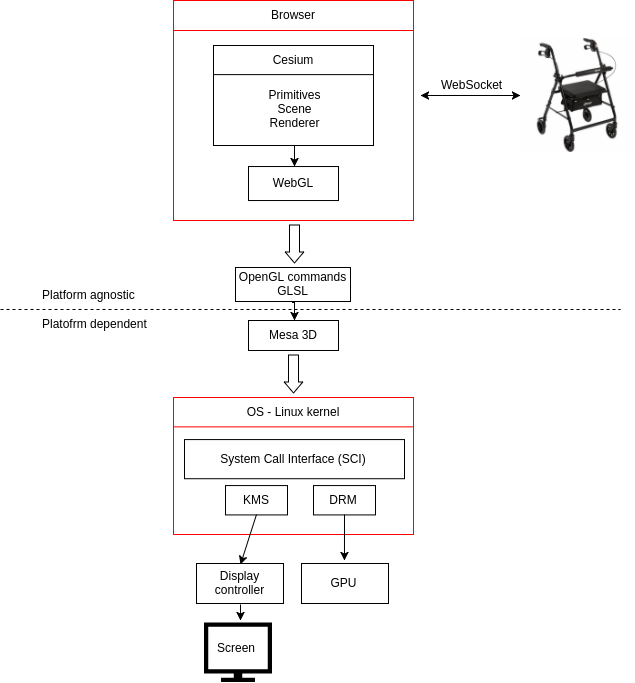
\includegraphics[width=0.6\linewidth]{system_architecture.png}}
    \caption{The FriWalk's system architecture.}
    \label{img:system_arch}
\end{figure}

As it is possible to see from Figure \ref{img:system_arch}, the first part includes
the walker assistant hardware, the browser running the
user interface (Google Chrome has been used in this study) and the component of
the OS which is responsible for implementing the OpenGL~\cite{woo1999opengl}
and the GLSL~\cite{marroquim2009introduction} libraries. On the other hand,
the platform dependent part includes the 3D graphics driver (eg. Mesa 3D for
Linux) and the OS kernel (eg. the Linux kernel). In the specific case of the
Linux kernel, it implements a System Call Interface (SCI) for interacting
with the Kernel Mode Setting (KMS)~\cite{linuxkms} and the Direct Rendering Manager
(DRM)~\cite{paul2000introduction}.


\subsection{Platform agnostic}
The 3D navigator application makes use of three pieces of information to move a
placeholder on the map: the \emph{latitude}, the \emph{longitude} and the
\emph{rotation}. These three values are not only the minimum amount of information
needed for the navigator to behave correctly, but also all the necessary.

From an high-level point of view, the walker assistant hardware can be regarded
as the portion of the system that is responsible for providing such data. Mooreover,
it can guarantee that data are available for the navigator at a fixed rate over
time using the WebSocket protocol~\cite{fette2011websocket}.
After receiving the data, the navigator properly moves the placeholder on the map.
This step can involves several operations, such as requesting a new tile for the
map, creating new 3D objects and so on. Consequently, the WebGL engine is responsible
for actually drawing the objects on the screen. A detailed description of how WebGL
behaves internally is given in Section \ref{sec:webgl}.

Finally, it is possible to say that the flow of information inside the platform
agnostic part of the system works as follows:
\begin{itemize}
    \item the FriWalk sends through a WebSocket the \emph{latitude}, the
        \emph{longitude} and the \emph{rotation} as a comma-separated string.
    \item the navigator running inside a browser receives the string, extracts
        the three values and uses them to build the objects needed to show the
        change on the screen.
    \item the framework powering the navigator actually performs the
        WebGL function calls.
    \item the graphical engine implemented inside the browser translates the WebGL
        function calls into generic OpenGL and GLSL commands, which are directly
        feeded to the graphical driver.
    \item the graphical hardware takes care of showing the scene on the screen.
\end{itemize}


\subsection{Platform dependent} \label{sec:platform_dependent}
This part of the system architecture highly depends on the operating system
running on the machine under test. In this work, a Linux-based OS (ie.
Ubuntu\footnote{\url{https://www.ubuntu.com}.})
has been used. Therefore the description may not fit, fully or partially, to
other operating systems like Apple Mac OS X, Microsoft Windows or other Linux
distributions.

The implementation of the OpenGL standard, the Mesa 3D Graphics Library. 
Graphics device drivers are implemented using two components: a User-Mode Driver
(UMD) and a Kernel-Mode Driver (KMD). The first can be seen as the interface
that can be used by other programs, while the second one directly interacts
with the KMS to set the display settings and with the DRM kernel subsystem
interfacing with the GPU(s). Starting from the 4.2 version of the Linux kernel,
multiple graphics drivers (eg. Mesa and AMD Catalyst) can share the same kernel
mode driver.


\section{Linux 3D graphics stack}
First it has to be underlined that this thesis refers only to the 3D part of the
graphics stack. This means that the window manager needs to ask the X11 server
only for the handle to a portion of the screen (i.e. the window).
3D graphics primitives do not need to interact any more with the X11 server. This
is needed to bypass the client-server architecture of X11 which is not suitable for
real-time 3D graphics and rendering, since it would have introduced more layers
of communication, delays and a high level of unpredictability.
This architecture is called
Direct Rendering Infrastructure (DRI)~\cite{paul2000introduction} and it is
necessary to overcome the scenario where only the X server is allowed to access
the graphics hardware. Moreover, DRI is composed by a user-space and a kernel-space
(ie. the DRM) part. This provides the building blocks that allow userspace applications
to directly access the graphics hardware in an efficient and safe way.
In addition, the DRM is a key component for the navigator application to achieve
hardware-accelerated 3D rendering and to manage video memory in Mesa.

As briefly described in Section \ref{sec:platform_dependent}, the Linux graphics
stack is quite complex and consists of many different layers in different parts
of the OS. The main ones are: the Mesa 3D Graphics Library, the System Call
Interface, the Kernel Mode Setting and the Direct Memory Manager.
As it is possible to see from Figure \ref{img:linux_graphics_stack}, the DRM and 
the display server belongs to the windowing system (eg. X11 or Wayland~\cite{wayland}) 
and it is not strictly necessary for applications directly using OpenGL function
calls.
\begin{figure}[!htb]
    \center{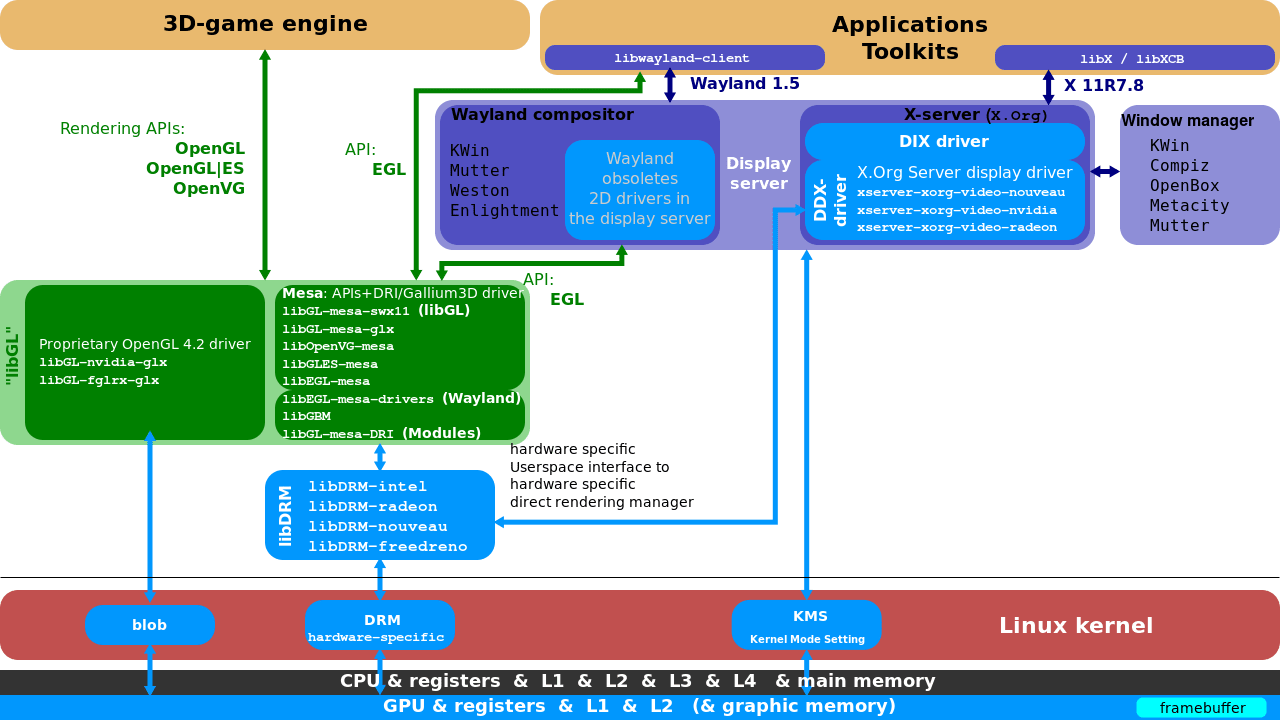
\includegraphics[width=0.75\linewidth]{linux_graphics_stack.png}}
    \caption{Illustration of the Linux graphics stack~\cite{fig_linux_graphics_stack}.}
    \label{img:linux_graphics_stack}
\end{figure}

Another key component is Mesa, a free and open-source implementation of the
OpenGL specification allowing
programs to output accelerated 3D graphics inside the Linux environment. Fortunately,
DRI is conceived to run without the brokering of the X server, but it is still
needed to allocate to Mesa a surface on the display to output to. Moreover, from
an high-level perspective the communication between Mesa and the GPU works by
exchanginc commands (eg. ``draw a point'') and data (eg. ``the coordinates of the
point and its color'') that are copied to a buffer shared with the graphics hardware.


\section{WebGL} \label{sec:webgl}
WebGL is a Javascript standard API for rendering 3D graphics within any compatible
desktop or mobile web browser\footnote{A compatibility table for all the most
common browsers can be found at the following link: \url{http://caniuse.com/#feat=webgl}.}
without any external program or toolkit. WebGL programs are composed of two parts
of code: some Javascript code, that can be mixed with any other part of a standard
HTML page which is executed by the browser, and some shader code, which is written 
in the OpenGL Shading Language (GLSL) and it is executed directly by the GPU.
WebGL APIs and are exposed to the Javascript engine of the browser through the
HTML5 canvas element. Moreover, this technology is based on the OpenGL for Embedded
Systems (ES),
which is a subset of standard OpenGL library and it is both
royalty-free and open-source\footnote{The WebGL source code can be found on GitHub
at the following link: \url{https://github.com/KhronosGroup/WebGL}.}.

In the last few years a lot of frameworks and utility libraries have been developed
and the huge capabilities of these 3D graphics APIs become visible to everybody.
A lot of libraries have been built upon WebGL to render scenes and 3D objects, such
as BabylonJS~\cite{babylon3d}, three.js~\cite{cabello2010three}, and 
Cesium~\cite{cozzi20113d} (see Section \ref{sec:cesium} for a more detailed description).
Moreover, there also has been a rapid emergence~\cite{parisi2014programming} of
game engines exploiting this technology like the Unreal Engine~\cite{games2007unreal}
and Unity~\cite{engine9unity}.

The reason why the 3D navigator developed in this work uses a framework built on
WebGL is that it is, at the time of writing, the only open-source alternative to
build 3D maps inside a browser. This choiche permits to write Javascript source
code to develop the application and, at the same time, to exploit the power of
a GPU using a framweork that takes care of implementing the shaders programs.
To be more precise, looking at the whole system architecture shown in Figure
\ref{img:system_arch}, WebGL is a technology that lie inside the browser
(in this specific case Google Chrome and its Skia\footnote{\url{https://skia.org}.}
graphics engine). The browser is the one responsible for communicating with
the actual implementation of OpenGL, which is Mesa in this case study.


\section{Cesium framework} \label{sec:cesium}
Cesium\footnote{\url{https://github.com/AnalyticalGraphicsInc/cesium}.} is an
open-source JavaScript library for building 3D globes and maps.
It is one of the leading technologies in the
field and its main characteristic is to achieve the ``best possible performance,
precision, visual quality, platform support, community, and ease of use''.
As previously described in Section \ref{sec:webgl}, it is one among a wide
possibility of frameworks for building interactive 3D maps. Cesium is chosen to
build the core of the navigator application for its outstanding performances,
its well written documentation and because it is also very easy to use. This last aspect
may not seem so important at a first glance; on the other hand, when dealing with
complex systems like the FriWalk it is very important to wisely choose all its building
blocks so that they can be successfully integrated to build the system as a whole
final product. Moreover, Cesium is actively developed and maintained by a company
whose main interest is delivering the best possible library for powering its
map-based software.

\subsection{Cesium's renderer architecture}
One of the most important features of the Cesium framework is its custom WebGL engine
called \emph{Renderer}.
It is built on the author's previous experience developing
other 3D globes libraries, which is explained in very detail in~\cite{cozzi20113d},
and it is responsible for collecting every interaction with WebGL in a single place.

Instead of scattering WebGL function calls all over the library, the centralization
of the Renderer has many and important benefits. First of all, it makes the
library very easy to use from the developer point of view, since it acts as an
intermediate layer of abstraction with respect to the plain WebGL calls. Furthermore,
it allows Cesium to build its runtime shader pipeline and its GLSL library. Last
but not least, optimizing the Renderer code through caching techniques allows
to highly improve performances allowing every other part of the framework to
benefit from it. As it is possible to see from Figure \ref{img:cesium_renderer},
the Renderer is composed of the following main parts:
\begin{itemize}
    \item the \emph{VertexArray} is a container of vertex attributes and indices
        which are stored in some internal buffers to reduce to the minimum the
        number of WebGL calls.
    \item the \emph{RenderState} includes all the WebGL functions states needed to
        perform a draw call. For example, it contains depth, blending and stencil
        states,
    \item the \emph{ShaderProgram} is a compiled/linked program with all its
        uniform matrix operations.
    \item the \emph{FrameBuffer} is a container for textures/rendererbuffer
        attachments which is the actual target of a draw call.
\end{itemize}

\begin{figure}[!htb]
    \center{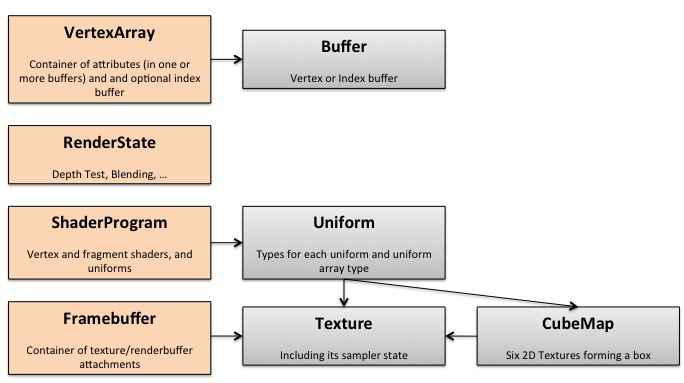
\includegraphics[width=0.55\linewidth]{cesium_renderer.jpg}}
    \caption{The components inside Cesium's Renderer~\cite{fig_cesium_renderer}.}
    \label{img:cesium_renderer}
\end{figure}

When Cesium executes a command it first binds the framebuffer (if it is different
from the previous command), then it applies the renderer states which are different
from the ones used in the last execution. Afterwards it binds\footnote{This step may
involve compiling and/or linking the shader code.} the shader program and finally it
issues a \emph{drawElements} or a \emph{drawArray} call.

Of course the Renderer is a major peculiarity of this library, but it is still only
one of its components. The Renderer uses the \emph{Scene} object to allocate and
create the WebGL resources needed for Cesium.
\begin{figure}[!htb]
    \center{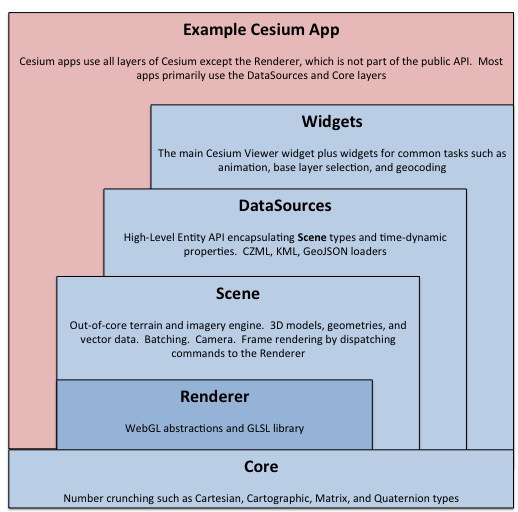
\includegraphics[width=0.45\linewidth]{cesium_stack.jpg}}
    \caption{All the components of the Cesium library~\cite{fig_cesium_renderer}.}
    \label{img:cesium_stack}
\end{figure}

Thus, as it is possible to see from Figure \ref{img:cesium_stack},
the Renderer is just a portion of the Scene component that is the ``real'' 3D
terrain and imagery engine.

Finally, as it is possible to see from Figure \ref{img:cesium_pipeline},
Cesium has a classic animate/update/render pipeline.
\begin{figure}[!htb]
    \center{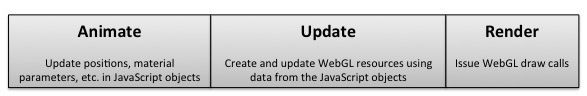
\includegraphics[width=0.6\linewidth]{cesium_pipeline.jpg}}
    \caption{The internal pipeline used in the Cesium framework~\cite{fig_cesium_pipeline}.}
    \label{img:cesium_pipeline}
\end{figure}

The \emph{animate} step involves all the aspects of building each object (eg.
textures, material properties etc.) that is later rendered without interacting with
WebGL. The \emph{update} step allocates and updates all the resources needed by
WebGL using the JavaScript objects created in the previous step. Eventually, the
\emph{renderer} phase actually issues the draw calls. All the available APIs
offered by Cesium can be found in~\cite{cesiumapi}.


\section{Goole Chrome's architecture}
As previously mentioned in Section \ref{sec:friwalk_architecture}, Google Chrome
is the browser chosen for the work of this thesis. This section aims at explaining
how Google Chrome is structured internally and how it interacts with the graphics
system. Since the Chromium project, which is the core part of Google Chrome, is
in rapidly and coutinuously evolving, everything that is written in this section
has to be considered the state of the art architecture at the time of writing.

Traditionally, web browsers only relied on the CPU for all the workload produced
by the page load. Nowadays GPUs (dedicated or integrated) are a very common piece
of hardware that almost every computer and smartphone owns. Hence a lot of attention
has been payed to the ability of graphics hardware of compositing web pages content
much faster with respect to the CPUs. Exploiting GPUs in a web
browser not only allows to use specific hardware for drawing pixels, but also to
enhence the parallelism between CPU and GPU that can work together for building
a very optimized rendering pipeline.

To better understand how GPU comes into play inside the architecture of Google
Chrome, the notion of \emph{compositor}~\cite{gpucompositing} has to be described first.
The compositor is a piece of software inside the browser that coordinates the frame
lifecycles and it manages the internal graphics data structures. The compositor
is allowed to use the GPU to perform the drawing steps. In this hardware-accelerated
architecture, compositing happens directly on the GPU via calls to the specific 3D
APIs implemented by the OS instead of communicating with the renderer process via
Inter Process Communication (IPC).
Having said that, it is crucial to explain how the renderer process issues
commands to the GPU. The browser is conceived to be multi-process, but
there is only one dedicated process for this task: the so called \emph{GPU process}.
The existance of this highly specialized process is a design decision made by Google's
engineers especially (but not only) for security concenrns. This is due to the
sandbox protecting each renderer process in Chrome, which means that it cannot
directly issue calls to the system or to the 3D graphics APIs
made available by the host OS (eg. OpenGL). For this reason it is the GPU process' job
to take care of this part of the rendering pipeline, since it is specifically
designed to provide access to the system's 3D graphics APIs from within the renderer
process ``jail''.
As it is possible to see from Figure \ref{img:chrome_gpu_compositing}, Chrome's
interaction with the GPU happens via a client-server model which is very similar
to the one used by X11.
\begin{figure}[!htb]
    \center{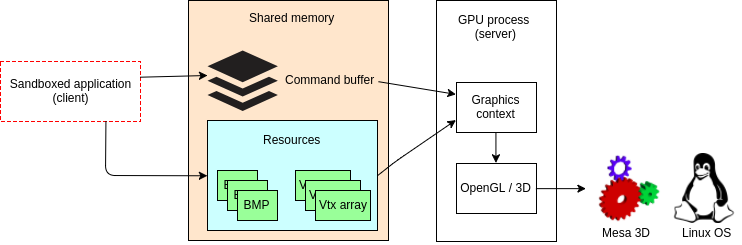
\includegraphics[width=0.8\linewidth]{chrome_gpu_architecture.png}}
    \caption{Google Chrome's GPU compositing.}
    \label{img:chrome_gpu_compositing}
\end{figure}

The flow of information works as follows:
\begin{itemize}
    \item the \emph{client} (ie. some code running inside the renderer process) serializes
        the calls for the system's 3D graphics (eg. WebGL calls) into a ring buffer called
        \emph{command buffer}~\cite{gpucommandbffer}. The data structure is basically a
        portion of memory which is shared between itself and the server counterpart of
        the architecture.
    \item the \emph{server} (ie. the GPU process/service) runs in a less restrictive sandbox
        and it is allowed to access the 3D APIs available on the system (eg. OpenGL via Mesa 3D).
        It takes the serialized commands which are into the buffer, it parses them and finally
        it issues the graphics calls to the driver.
\end{itemize}

The reason behing the usage of a shared storage between the client and the server to implement
the command buffer is to optimize the passage of large resources, such as bitmaps,
textures and vertex arrays. Another important aspect of this design choice is
portability. This means that, from the point of view of the client, there is (nearly) no
difference across different systems and OSs. Last but not least, the command buffer
structure allows to achieve very high performances; the client can write commands
very fast without any communication with to server and, once in a while,
it tells the server that it has written more commands into the buffer.
From the implementation perspective, the command buffer is a shared portion of
memory collecting the commands a client puts into it. Consequently the client
communicates to the GPU process how much data it wrote into that buffer so that
the GPU process can read, parse, validate and execute these commands.

Another important issue that had to be addressed is the syncronization between different
command buffers sharing some data (eg. textures). This can be enforced inserting
\emph{sync points} and can prevent a lot of data duplicates.
For example it is possible to insert a sync point on buffer A
to wait for another sync point in buffer B, thus ensuring that commands appended to
B will not run before the ones inserted in A before the sync point. This feature
is very useful every time multiple buffer are sharing some data.

To summarize the key points of the Google Chrome architecture, the single GPU
process per browser instance has multiple benefits. First of all it strengthen
security, since the rendering logic is inside a sandboxed renderer and the interaction
with the 3D graphics APIs is limited to one single process. Moreover, it allows
the entire browser instance not to crash if the GPU service does not work properly.
Finally it brings all the benefits of parallelism, where the renderer can issue
commands very quickly leaving the GPU process the hard work to actually run them
using the graphics hardware available on the system. This clearly allows to better
exploit the multi-core architectures so that the CPU and the GPU can work at the
same time.

        %!TEX root=../thesis.tex
\chapter{Problem definition} \label{cha:problem_definition}

Problem definition

        %!TEX root=../thesis.tex
\chapter{A Real-Time model for WebGL} \label{cha:rt_model}

WebGL is a relatively new technology that enables hardware-accelerated web
contents. Moreover, in the last few years Virtual Reality (VR) has became
another very popular research topic. The Mozilla Foundation is actively working
for bringing VR technologies to the web by means of WebVR~\cite{mozvr}. WebVR is
``an open specification that makes it possible to experience VR'' inside a web
browser, whose main goal is to make VR experiences easier, regardless of the
device used. This specification is available
via different frameworks like Mozilla's A-Frame~\cite{aframe}, which allows
to build virtual reality scenes inside the browser using only HTML and JavaScript
code.\\
This may seem a very different field with respect to the one of this
thesis, but what makes A-Frame similar to Cesium is how they exploit WebGL to
interact with the GPU to achieve hardware acceleration. In this sense it is
reasonable to compare VR and 3D-maps web technologies since they both use WebGL
in their core. Furthermore, virtual reality applications are even more
performance-demanding from the real-time point of view, since even relatively
small latencies (ie. in the order of tenths of milliseconds) can make a product
completely unusable and annoy the human eyesight.


\section{Assumptions} \label{sec:assumptions}
First of all, all the experiments presented in this thesis are run on a Dell
Inspiron 15R 5521 notebook\footnote{\url{http://www.dell.com/us/dfh/p/inspiron-15r-5521/pd}.},
whose hardware specifications are shown in Table \ref{tab:notebook_specs}.
Since 3D graphics performance highly depends on the GPU installed on the system,
the results presented in Chapter \ref{cha:experiments} are likely to be overtaken
if better graphics hardware (eg. a more powerful dedicated GPU) is installed.
\begin{table}[!htb]
    \centering
    \caption{The test machine hardware specifications.}
    \label{tab:notebook_specs}
    \begin{tabular}{|l|l|l|l|}
    \hline
    \multicolumn{1}{|l|}{\textbf{CPU}} & \multicolumn{1}{l|}{\textbf{GPU (integrated)}} & \multicolumn{1}{l|}{\textbf{RAM}} & \multicolumn{1}{l|}{\textbf{Hard drive}} \\ \hline
    Intel i7 3537U & Intel® HD Graphics 4000 & 8GB DDR3 & Samsung 850 Evo 250GB \\ \hline
    \end{tabular}
\end{table}

Another important aspect is how tests are conceived. As it is always the case in
real-time analysis, the worst possible scenario is the one of interest for
computing the WCET of a task. To achieve this situation in the test application,
Google Chrome is always run from scratch with only one active tab. Moreover, the browser
is forced not to cache any part of the JavaScript application code but,
at the same time, it is essential to eliminate the map retrival time.
Usually map tiles are
downloaded via HTTP using the REST APIs a terrain server exposes to the clients.
Even the time the navigator takes to download a small portion of the terrain
can be orders of magniture bigger than all the rest of the response/computation time.
Hence, this objective is obtained allowing the browser to locally save the
tiles downloaded during a ``warm-up'' phase. This allows to significantly lower
the map retrival time during the ``real'' experiment without jeopardizing the
timings of the entire trace.

Finally, picking timestamps during the execution of a piece of software can bias
the correctness of the data. This is another point that has to be
taken into account during any type of analysis involving time measurements like
the one presented in this work. In simple terms, measuring time takes time and
it does not come for free.


\section{Tools used}
This section presents the tools used to profile the test application and to pick
the timings needed for the experiments shown in Chapter \ref{cha:experiments}.
Even though the description reflects the specific usage in this work, these
software toolkits can be applied to a wide variety of fields and scenarios.

\subsection{Web Tracing Framework} \label{sec:wtf}
The Web Tracing Framwork (WTF)~\cite{wtf} is composed of a set of tools for
instrumenting, analyzing and visualizing web application execution traces.
It is an extensible framework able to capture and to replay HTML5 canvas elements
along with its WebGL content. In this way it is possible to implement a plugin for
this framework that is specific for the purpose of the application under test.
Furthermore, a wide set
of methods and events can be tracked out-of-the-box for preliminar investigations.

WTF is a very good toolset for an high-level analysis of web applications,
providing easy code instrumentation to track only what is truly interesting for the developer.
The usual work-flow is the following. First the events to be traced 
are selected, either from a predefined set or specific code instrumentation can be
inserted inside the source code using the framework's APIs. After that, the application's source code
has to include four the proper function calls to control the tracing mechanism.
An example of application source code is the following:
\begin{lstlisting}[caption=Usage example of the Web Tracing Framework., language=JavaScript,
  label=code:wtf_example]
  let wtfOptions = { ... }; // customize WTF behaviour
  wtf.trace.prepare(wtfOptions);
  /* application initialization */
  wtf.trace.start(); // start profiling
  /* code to be traced goes here */
  wtf.trace.snapshot("file://trace"); // save trace to file
  wtf.trace.stop(); // stop profiling
\end{lstlisting}

After taking a snapshot of the current trace (line 6, code snippet \ref{code:wtf_example})
and stopping capturing data (line 7), the trace is exported in a
compressed format that can be manipulated using some CLI
scripts\footnote{\url{https://github.com/google/tracing-framework}.} to export
data in Comma Separated Values (CSV) format. Otherwise the results can be visualized
thanks to the proper web
page\footnote{\url{http://google.github.io/tracing-framework/bin/app/maindisplay.html}.}.

Another highlight is its extendibility. In this way the developer can either
profile the application using the default events emitted by the browser or can 
directly instrument the source code to track only very specific parts. Basically, this
allows to measure nearly everything that is accessible from JavaScript, even
though it may not be enough in some situation.

Finally, a post-process task is required to get insights from the raw data.
The CSV exported by the Web Tracing Framweork has the following structure:
\begin{equation*}
    <time,\,value,\,total\_time,\,own\_time,\,arguments>
\end{equation*}

where:
\begin{itemize}
    \item \emph{time}: it is the amount of time (in milliseconds) elapsed from the
        \emph{wtf.trace.start()} function call.
    \item \emph{value}: it is the function name that is traces. More specifically this
        value is a string composed by\\
        ''\([context\_name]\#[function\_name]\)''.
    \item \emph{total\_time}: it is the time taken to complete the current invocation
        of the function (in milliseconds) along with any other function that
        is called.
    \item \emph{own\_time}: it is how long it took to complete the current invocation
        of the function (in milliseconds) without including any function called by
        the current one.
    \item \emph{arguments}: they all the arguments (with values) that are passed
        to the \emph{value} function.
\end{itemize}

Clearly, being the computaton of latencies the main aim this framework, the most
relevant fields to be later analyzed are the \emph{time}, the \emph{total\_time}
and the \emph{own\_time} values.


\subsection{Chrome's trace event profiler}
The other foundamental tool used to trace the test application is the trace
event profiler embedded into Google Chrome. This is another important reason why
Chrome is preferred as browser for the entire work, since it allows to diagnose
performance issues and to see what Chrome is really doing ``under the surface''.
This tool is available by default in any build of Google Chrome typing
\emph{chrome://tracing} inside the main URL bar.

This profiler ``records all the C++ and JavaScript method signatures in a
hierarchical view for each thread in each process'' of the browser. This results
in a huge amount of information, but it helps to identify performance bottlenecks
and to spot any kind of event happening to the browser instance. Hence, this tool
allows to
better analyze a web application, collecting all the events occuring when the
application is running starting from the renderer processes IPC up to every single
function that is executed by the GPU process.

Sometimes it may be necessary
to run Chrome with some particular command line flag in order to enable the
``debugging mode'' for some feature. For example, the \emph{--enable-skia-benchmarking}
flag is needed for profiling the Skia graphics engine. These additional flags
are not used by default since users do not need to profile the entire browser
all the time and thus, skipping some instruction inside the browser's source code
can result in better response times and navigation fluency.

Consequently, it is possible
to say that this event profiler perfectly fits a low-level analysis of everything
that happens inside the complex architechture of Google Chrome.
As it is possible to see from Figure \ref{img:chrome_event_profiler}, this tool
is capable not only to acquire data from the browser but also to visualize them
as flame graphs~\cite{gregg2016flame}.
\begin{figure}[!htb]
    \center{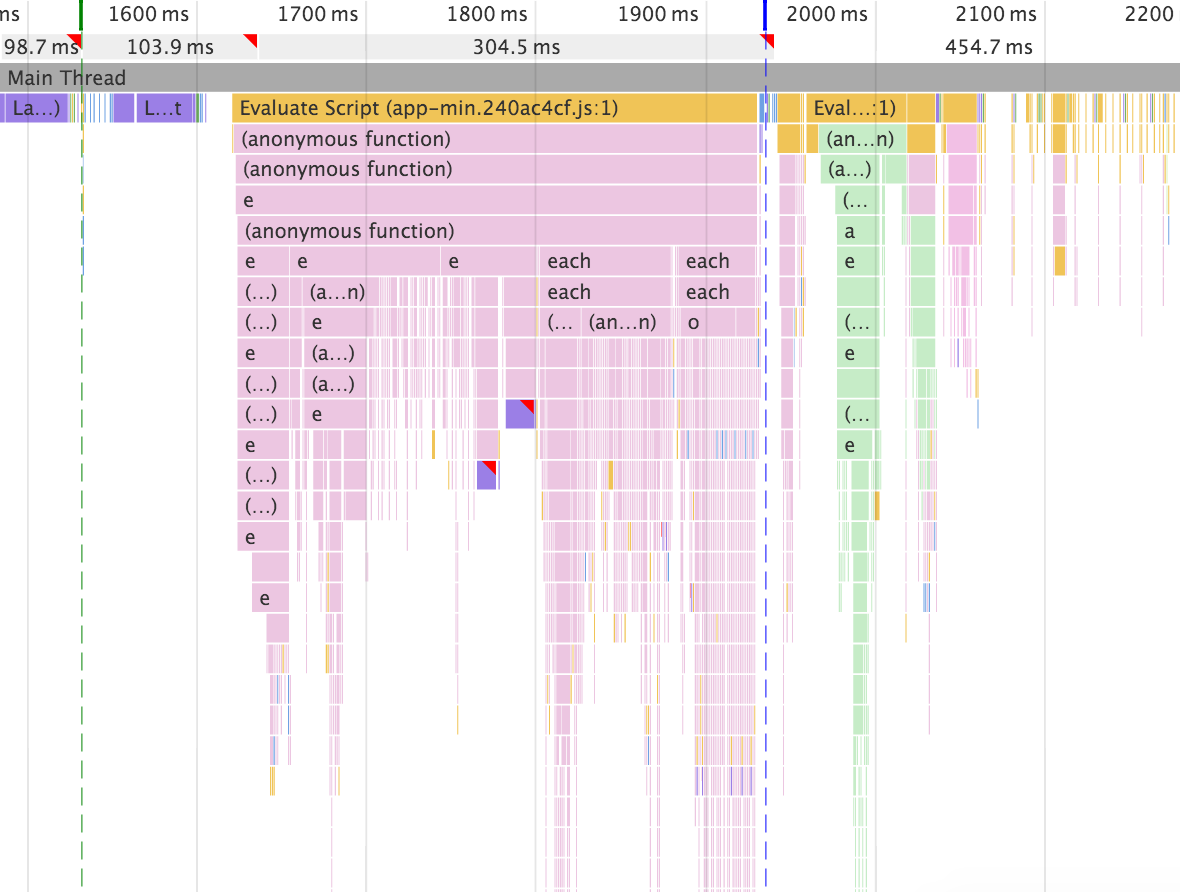
\includegraphics[width=0.47\linewidth]{chrome_event_profiler.png}}
    \caption{The viewer user interface for the Chrome event profiler.}
    \label{img:chrome_event_profiler}
\end{figure}

The output format of this tool is a JavaScript Object Notation (JSON) file with
several fieds. The ones of interest for the purpose of this work are the following:
\begin{lstlisting}
{
  "pid": 5782,
  "tid": 5782,
  "ts": 3951728304,
  "ph": "X",
  "cat": "gpu",
  "name": "GpuCommandBufferStub::OnAsyncFlush",
  "args": { ... },
  "dur": 113,
  "tdur": 112,
  "tts": 1213475
}
\end{lstlisting}

where:
\begin{itemize}
    \item \emph{pid}: it is the process id of the process outputting the event.
    \item \emph{tid}: it is the thread id for the thread outputting the event.
    \item \emph{ts}: it is the tracing clock timestamp (in microseconds), meaning
        the amount of time elapsed from the tracing start.
    \item \emph{ph}: it is the event type that is recorded. This is a single character
        that depends on the type of event being tracked\footnote{A complete list
        of the type of events available can be found at the following link:
        \url{https://docs.google.com/document/d/1CvAClvFfyA5R-PhYUmn5OOQtYMH4h6I0nSsKchNAySU/}.}
    \item \emph{cat}: it represents the event category. This a list used to hide
        events from the Trace Viewer user interface.
    \item \emph{name}: it is the name of the event.
    \item \emph{args}: this contains any argument that is provided to the event/function
        call.
    \item \emph{dur}: it specifies the tracing clock duration of complete events
        (in microseconds).
    \item \emph{tdur}: it specifies the thread clock duration of complete events
        (in microseconds).
    \item \emph{tts}: it specifies the thread clock timestamp of the event (in
        microseconds).
\end{itemize}

Among all the abovementioned values, the most important ones during the experiments
are the \emph{ts} and the \emph{tdur}; they allow to specify when an event has been
fired and for how much time the thread computing that function run.


\section{Profiling and analysis procedures} \label{sec:procedure}
Some extra work has been done to provide a very convenient way
for capturing data with the tool presented in the previous section. A program
simulating the FriWalk hardware has been developed to send the values for position
and rotation to the web
interface via the WebSocket protocol. This is useful to emulate the behaviour of
a portion of the system architechture (see Figure \ref{img:system_arch}) that was
not always available during the development of this thesis.

Even from the very first test with WTF it became clear that the system under
test is as complex as the problem this thesis aims to solve. Therefore, the hard
problem of profiling the entire navigator application is split into many simpler
parts. Moreover, the navigator is traced from its startup until the first new
position is sent by the FriWalk and it is displayed on the screen. This idea of reducing the
amount of workload to the minimum allows to better concentrate on fewer and more
specific data outputted by the two tracing tools. Hence, four different scenarios
have been implemented:
\begin{itemize}
    \item the complete navigator application.
    \item a ``camera-only'' mode; in this scenario there is no physical placeholder
        to be moved on the map and only the user's camera is moved.
    \item a ``no-map'' mode; in this scenario the map is completely
        excluded from the application, meaning that no tail for the terrain is
        downloaded.
    \item a ``redraw'' mode; this is a scenario simulating a walker that remains
        always stationary in the same position.
\end{itemize}

All the scenarios mentioned above aims at simplifying the post-processing
analysis and to focus on the different parts of the navigator. For example, the
``no-map'' mode is conceived to get rid of the map but, at the same time, to keep
all the base functionalities of the navigator. To some extent, the partial traces
obtained from all these scenarios can be utilized to compare each other and spot
their similarities and/or differencies.

Finally, a Python script is used to split and to graphically display the
timings extracted from the traces. Having a visual representation is often very
useful to better undestand what is happening as the time passes inside the application
trace.

        %!TEX root=../thesis.tex
\chapter{Experiments} \label{cha:experiments}


\begin{table}[!htb]
    \centering
    \caption{WebGL functions-to-groups mapping.}
    \label{tab:webgl_func_mapping}
    \begin{tabular}{|l|l|l|}
        \hline
        \textbf{Initialization} & \textbf{Modify data} & \textbf{Display} \\ \hline
        bindBuffer/bindFramebuffer & uniformMatrix3fv/uniformMatrix4fv & drawElements \\
        enable/disable & uniform[1\(\vert\)2\(\vert\)3\(\vert\)4][f\(\vert\)i\(\vert\)iv\(\vert\)fv] & drawArray \\
        viewport & bindTexture/activeTexture &  \\
        clear/clearColor & bufferSubData &  \\
        cullFace &  &  \\
        depthCompare &  &  \\
        useProgram &  &  \\
        colorMask &  &  \\
        \hline
    \end{tabular}
\end{table}

\begin{figure}[!htb]
    \center{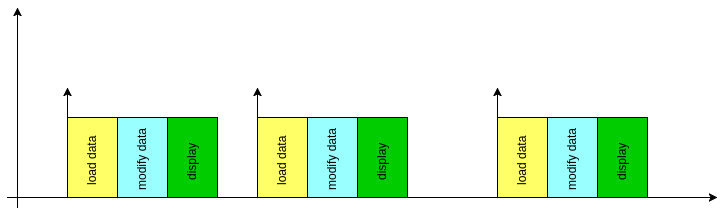
\includegraphics[width=0.6\linewidth]{call_arrival.png}}
    \caption{The function calls arrival approximate model with different groups.}
    \label{img:call_arrival}
\end{figure}

        %!TEX root=../thesis.tex
\chapter{Conclusion and future work} \label{cha:conclusion}

Adopting the Markov Computation Time Model to study the behaviour of a web
application which heavily use WebGL is feasible.
The outcomes presented in Section \ref{sec:mctm_results} show that it is
reasonable to split the original computation time trace into two states, since
the output model is always conservative.
However, the values belonging to each modes are not highly correlated but they
are not independent as they should be in principle.
This may be a problem in the logic of the HMM decoder algorithm. In the specific
case of this work, the classification phase splits the original trace into two
states (Figure \ref{img:mctm_2_states}) whose CDFs are clearly distinct. On the
other hand, if a system composed of three modes is considered, two out of three
CDFs are completely overlapped. Hence, two is the number of states that best
fits the MCTM.

As future work, it is possible to switch from the ``raw'' computation times taken
into consideration in this thesis to ``per-frame'' values. This can be done
summing the computation times belonging to the same frame and it allows to study
the WebGL rendering performance from a slightly different standpoint.
Furthermore, the work of this thesis is not bound only to the specific
application under test and it can be easily extended to study the performances
of any piece of software running inside a web browser. This flexibility allows
the team working on the ACANTO project to run the entire analysis on the
specific hardware available on the FriWalk. In addition to this, another
challenging improvement is to modify Cesium's rendering pipeline to introduce
the concept of priority queues for the WebGL primitives. In this way it would
be possible to render the ``most important'' parts of the scene first (e.g., near
the user's position) and to delay the ``less important'' ones.

    \endgroup

    % bibliografia in formato bibtex
    % aggiunta del capitolo nell'indice
    \addcontentsline{toc}{chapter}{Bibliography}
    % stile con ordinamento alfabetico in funzione degli autori4
    \newpage % leave this here
    \bibliographystyle{plain}
    \bibliography{biblio}

    % appendix
    %\titleformat{\chapter}
    %    {\normalfont\Huge\bfseries}{Appendix \thechapter}{1em}{}
    % sezione Allegati - opzionale
    %\appendix
    %\chapter{Titolo primo allegato}

Lorem ipsum dolor sit amet, consectetur adipiscing elit. Donec sed nunc orci. Aliquam nec nisl vitae sapien pulvinar dictum quis non urna. Suspendisse at dui a erat aliquam vestibulum. Quisque ultrices pellentesque pellentesque. Pellentesque egestas quam sed blandit tempus. Sed congue nec risus posuere euismod. Maecenas ut lacus id mauris sagittis egestas a eu dui. Class aptent taciti sociosqu ad litora torquent per conubia nostra, per inceptos himenaeos. Pellentesque at ultrices tellus. Ut eu purus eget sem iaculis ultricies sed non lorem. Curabitur gravida dui eget ex vestibulum venenatis. Phasellus gravida tellus velit, non eleifend justo lobortis eget. 

\section{Titolo}
Lorem ipsum dolor sit amet, consectetur adipiscing elit. Donec sed nunc orci. Aliquam nec nisl vitae sapien pulvinar dictum quis non urna. Suspendisse at dui a erat aliquam vestibulum. Quisque ultrices pellentesque pellentesque. Pellentesque egestas quam sed blandit tempus. Sed congue nec risus posuere euismod. Maecenas ut lacus id mauris sagittis egestas a eu dui. Class aptent taciti sociosqu ad litora torquent per conubia nostra, per inceptos himenaeos. Pellentesque at ultrices tellus. Ut eu purus eget sem iaculis ultricies sed non lorem. Curabitur gravida dui eget ex vestibulum venenatis. Phasellus gravida tellus velit, non eleifend justo lobortis eget. 

\subsection{Sottotitolo}
Lorem ipsum dolor sit amet, consectetur adipiscing elit. Donec sed nunc orci. Aliquam nec nisl vitae sapien pulvinar dictum quis non urna. Suspendisse at dui a erat aliquam vestibulum. Quisque ultrices pellentesque pellentesque. Pellentesque egestas quam sed blandit tempus. Sed congue nec risus posuere euismod. Maecenas ut lacus id mauris sagittis egestas a eu dui. Class aptent taciti sociosqu ad litora torquent per conubia nostra, per inceptos himenaeos. Pellentesque at ultrices tellus. Ut eu purus eget sem iaculis ultricies sed non lorem. Curabitur gravida dui eget ex vestibulum venenatis. Phasellus gravida tellus velit, non eleifend justo lobortis eget. 


\chapter{Titolo secondo allegato}

Lorem ipsum dolor sit amet, consectetur adipiscing elit. Donec sed nunc orci. Aliquam nec nisl vitae sapien pulvinar dictum quis non urna. Suspendisse at dui a erat aliquam vestibulum. Quisque ultrices pellentesque pellentesque. Pellentesque egestas quam sed blandit tempus. Sed congue nec risus posuere euismod. Maecenas ut lacus id mauris sagittis egestas a eu dui. Class aptent taciti sociosqu ad litora torquent per conubia nostra, per inceptos himenaeos. Pellentesque at ultrices tellus. Ut eu purus eget sem iaculis ultricies sed non lorem. Curabitur gravida dui eget ex vestibulum venenatis. Phasellus gravida tellus velit, non eleifend justo lobortis eget. 

\section{Titolo}
Lorem ipsum dolor sit amet, consectetur adipiscing elit. Donec sed nunc orci. Aliquam nec nisl vitae sapien pulvinar dictum quis non urna. Suspendisse at dui a erat aliquam vestibulum. Quisque ultrices pellentesque pellentesque. Pellentesque egestas quam sed blandit tempus. Sed congue nec risus posuere euismod. Maecenas ut lacus id mauris sagittis egestas a eu dui. Class aptent taciti sociosqu ad litora torquent per conubia nostra, per inceptos himenaeos. Pellentesque at ultrices tellus. Ut eu purus eget sem iaculis ultricies sed non lorem. Curabitur gravida dui eget ex vestibulum venenatis. Phasellus gravida tellus velit, non eleifend justo lobortis eget. 

\subsection{Sottotitolo}
Lorem ipsum dolor sit amet, consectetur adipiscing elit. Donec sed nunc orci. Aliquam nec nisl vitae sapien pulvinar dictum quis non urna. Suspendisse at dui a erat aliquam vestibulum. Quisque ultrices pellentesque pellentesque. Pellentesque egestas quam sed blandit tempus. Sed congue nec risus posuere euismod. Maecenas ut lacus id mauris sagittis egestas a eu dui. Class aptent taciti sociosqu ad litora torquent per conubia nostra, per inceptos himenaeos. Pellentesque at ultrices tellus. Ut eu purus eget sem iaculis ultricies sed non lorem. Curabitur gravida dui eget ex vestibulum venenatis. Phasellus gravida tellus velit, non eleifend justo lobortis eget. 



\end{document}

%%%%%%%%%%%%%%%%%%%%%%%%%%%%%%%%%%%%%%%%%%%%%%%%%%%%%%%%%%%%%%%%%%%%%%%%%%
%% Nota
%%%%%%%%%%%%%%%%%%%%%%%%%%%%%%%%%%%%%%%%%%%%%%%%%%%%%%%%%%%%%%%%%%%%%%%%%%
%% Nella bibliografia devono essere riportati tutte le fonti consultate
%% per lo svolgimento della tesi. La bibliografia deve essere redatta
%% in ordine alfabetico sul cognome del primo autore.
%%
%% La forma della citazione bibliografica va inserita secondo la fonte utilizzata:
%%
%% LIBRI
%% Cognome e iniziale del nome autore/autori, la data di edizione, titolo, casa editrice, eventuale numero dell’edizione.
%%
%% ARTICOLI DI RIVISTA
%% Cognome e iniziale del nome autore/autori, titolo articolo, titolo rivista, volume, numero, numero di pagine.
%%
%% ARTICOLI DI CONFERENZA
%% Cognome e iniziale del nome autore/autori (anno), titolo articolo, titolo conferenza, luogo della conferenza (città e paese), date della conferenza, numero di pagine.
%%
%% SITOGRAFIA
%% La sitografia contiene un elenco di indirizzi Web consultati e disposti in ordine alfabetico.
%% E’ necessario:
%%   Copiare la URL (l’indirizzo web) specifica della pagina consultata
%%   Se disponibile, indicare il cognome e nome dell’autore, il titolo ed eventuale sottotitolo del testo
%%   Se disponibile, inserire la data di ultima consultazione della risorsa (gg/mm/aaaa).
%%%%%%%%%%%%%%%%%%%%%%%%%%%%%%%%%%%%%%%%%%%%%%%%%%%%%%%%%%%%%%%%%%%%%%%%%%
